\documentclass[a4paper,12pt]{article}
\usepackage{amsmath,amssymb,amsfonts,amsthm}
\usepackage{tikz}
\usepackage [utf8x] {inputenc}
\usepackage [T2A] {fontenc} 
\usepackage[russian]{babel}
\usepackage{cmap} 
\usepackage{gensymb}

% Так ссылки в PDF будут активны
\usepackage[unicode]{hyperref}

% вы сможете вставлять картинки командой \includegraphics[width=0.7\textwidth]{ИМЯ ФАЙЛА}
% получается подключать, как минимум, файлы .pdf, .jpg, .png.
\usepackage{graphicx}
% Если вы хотите явно указать поля:
\usepackage[margin=1in]{geometry}
% Или если вы хотите задать поля менее явно (чем больше DIV, тем больше места под текст):
% \usepackage[DIV=10]{typearea}

\usepackage{fancyhdr}

\newcommand{\bbR}{\mathbb R}%теперь вместо длинной команды \mathbb R (множество вещественных чисел) можно писать короткую запись \bbR. Вместо \bbR вы можете вписать любую строчку букв, которая начинается с '\'.
\newcommand{\eps}{\varepsilon}
\newcommand{\bbN}{\mathbb N}
\newcommand{\dif}{\mathrm{d}}

\newtheorem{Def}{Определение}


\pagestyle{fancy}
\makeatletter % сделать "@" "буквой", а не "спецсимволом" - можно использовать "служебные" команды, содержащие @ в названии
\fancyhead[L]{\footnotesize Термодинамика и молекулярная физика}%Это будет написано вверху страницы слева
\fancyhead[R]{\footnotesize ФМХФ МФТИ}
\fancyfoot[L]{\footnotesize \@author}%имя автора будет написано внизу страницы слева
\fancyfoot[R]{\thepage}%номер страницы —- внизу справа
\fancyfoot[C]{}%по центру внизу страницы пусто

\renewcommand{\maketitle}{%
	\noindent{\bfseries\scshape\large\@title\ \mdseries\upshape}\par
	\noindent {\large\itshape\@author}
	\vskip 2ex}
\makeatother
\def\dd#1#2{\frac{\partial#1}{\partial#2}}


\title{2.3.1 \\ Получение и измерение вакуума } 
\author{Егор Берсенев} 
\date{10 мая 2016 г.}

\begin{document}
	\maketitle
	\section{Цель:}
	\begin{enumerate}
		\item Измерение объемов форвакуумной и высоковакуумной частей установки.
		\item Определение скорости откачки системы в стационарном режиме, а также по ухудшению и по улучшению вакуума. 
	\end{enumerate}
	\section{Оборудование:}
		Вакуумная установка с манометрами: масляным, термопарным и ионизационным.
	\section{Теоретическая часть}
	Формула, выражающая скорость откачки газа из установки через предельный объем:
	\begin{equation}
		-V\mathrm{d}P = \left(P_{\text{пр}}W - Q_{\text{д}} - Q_{\text{н}} - Q_{\text{и}}\right)\mathrm{d}t
	\end{equation}
	При достижении предельного давления $\frac{\dif P}{\dif t}=0$, значит:
	\begin{equation}
	P_{\text{пр}}W = Q_{\text{д}} + Q_{\text{н}} + Q_{\text{и}}
	\end{equation}
	Обычно $Q_{\text{д}}, Q_{\text{н}}, Q_{\text{и}}$ можно считать постоянными. Тогда, проинтегрировав, получаем:
	\begin{equation}
	P = P_0\exp\left(-\frac{W}{V}t\right)
	\end{equation}
	Для газа, протекающего через трубу в Кнудсеновском режиме справедлива формула:
	\begin{equation}
		\frac{\dif(PV)}{\dif t} = \frac{4}{3}r^3\sqrt{\frac{2\pi RT}{\mu}}\frac{P_2-P_1}{L}
	\end{equation}
	Применим для газа, протекающего через трубу от установки к насосу.
	 \begin{equation}
	 С_{\text{тр}}=\frac{\dif V}{\dif t} = \frac{4}{3}\frac{r^3}{L}\sqrt{\frac{2\pi RT}{\mu}}
	 \end{equation}
	Пропускная способность кранов:
	\begin{equation}
		\nu = \frac{1}{4}Sn\bar{v} \implies C_{\text{отв}}= \frac{1}{4}S\bar{v} 
	\end{equation}
	\section{Экспериментальная установка}
    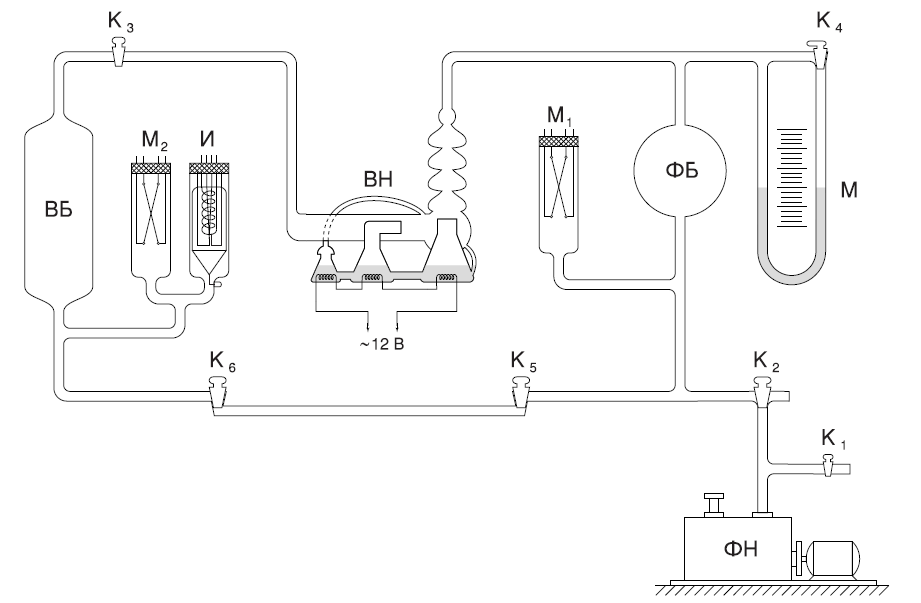
\includegraphics[width = 0.7\linewidth]{instrument1}
    
    ФБ – форвакуумный баллон
    
    ВН – высоковакуумный диффузионный насос
    
    ВБ – высоковакуумный баллон
   
    М – масляной манометр
   
    И – ионизационный манометр
  
    М1, M2 – термопарные манометры
  
    К1 --- К6 – соединительные краны
    
	
	\section{Ход работы}
	\subsection{Опредение объема форвакуумной и высоковакуумной частей установки}
	Проверим положение кранов, откроем кран К2, чтобы запустить в систему воздух, подождем 2 минуты, пока воздух заполнт всю установку.
	Между кранами К5 и К6 заперто $V_{\text{К5+К6+кап}}=60+\pm 3 \text{см}^3$ воздуха при атмосферном давлении. Откачаем систему до низкого вакуума и откроем кран. Воздух, запертый в кране заполнит объем форвакуумной части установки. Рассчитаем его. По масляному манометру $h_1 = 21, h_2 = 40 \implies\Delta h = 19$
	\[
	P_2 = \Delta h \cdot \rho \cdot g = 0.19\cdot885\cdot9.8 = 1647\, \text{Па} \implies V_{\text{фв}}=\frac{P_{\text{атм}}V_{\text{крана}}}{P_{\text{фв}}} = \frac{101325\cdot 0.06}{1647}=3.69 \pm 0.19 \,\text{л}
	\]
	
	Рассчитаем объем высоковакумной части. 
	\[
	P_3 = \Delta h \cdot \rho \cdot g = 0.105\cdot885\cdot9.8 = 910.6\, \text{Па} \implies V_{\text{фв+вв}}=\frac{P_{\text{атм}}V_{\text{крана}}}{P_{\text{фв+вв}}} = \frac{101325\cdot 0.06}{910.6}=6.676 \,\text{л} 
	\]
	\[ 
	V_{\text{вв}} = 6.676-3.69=2.986\pm0.16\,\text{л}
	\]
	
	Измерим предельное давление в системе: $P_{\text{пред}} = 3 \cdot 10^{-4}\,\text{торр}$ при $U = 30 \,\text{mA}$.
	
	Найдем ухудшение вакуума во времени по изменению показаний ионизационного манометра.
	\begin{center}
	\begin{table}[h]
		\begin{tabular}{l|l|l|l|l|l|l|l|l|l|l|l}
			$P\cdot 10^{-5}$, Торр  & 30 & 40 & 50 & 60 & 70 & 80 & 70 & 60 & 50 & 40 & 30 \\ \hline
			$t_1$, c              & 0 & 8.5 & 25.26 & 40.31 & 58.67 & 76.38 & 3.79 & 8.5 & 15.96 & 31.15 & 59.25 \\
			$t_2$, c              & 0 & 12.36 & 28.856 & 46.26 & 64.85 & 84.85 & 5.2  & 9.09 & 16.16 & 28.65 & 53.74 \\
			$\bar{t}$, c        & 0 & 10.43 & 27.06 & 43.29 & 61.76 & 80.62 & 4.5 & 8.8 & 16.06 & 29.90 & 56.50 \\
		\end{tabular}
	\end{table}
	\end{center}
	Построим графики:
	
	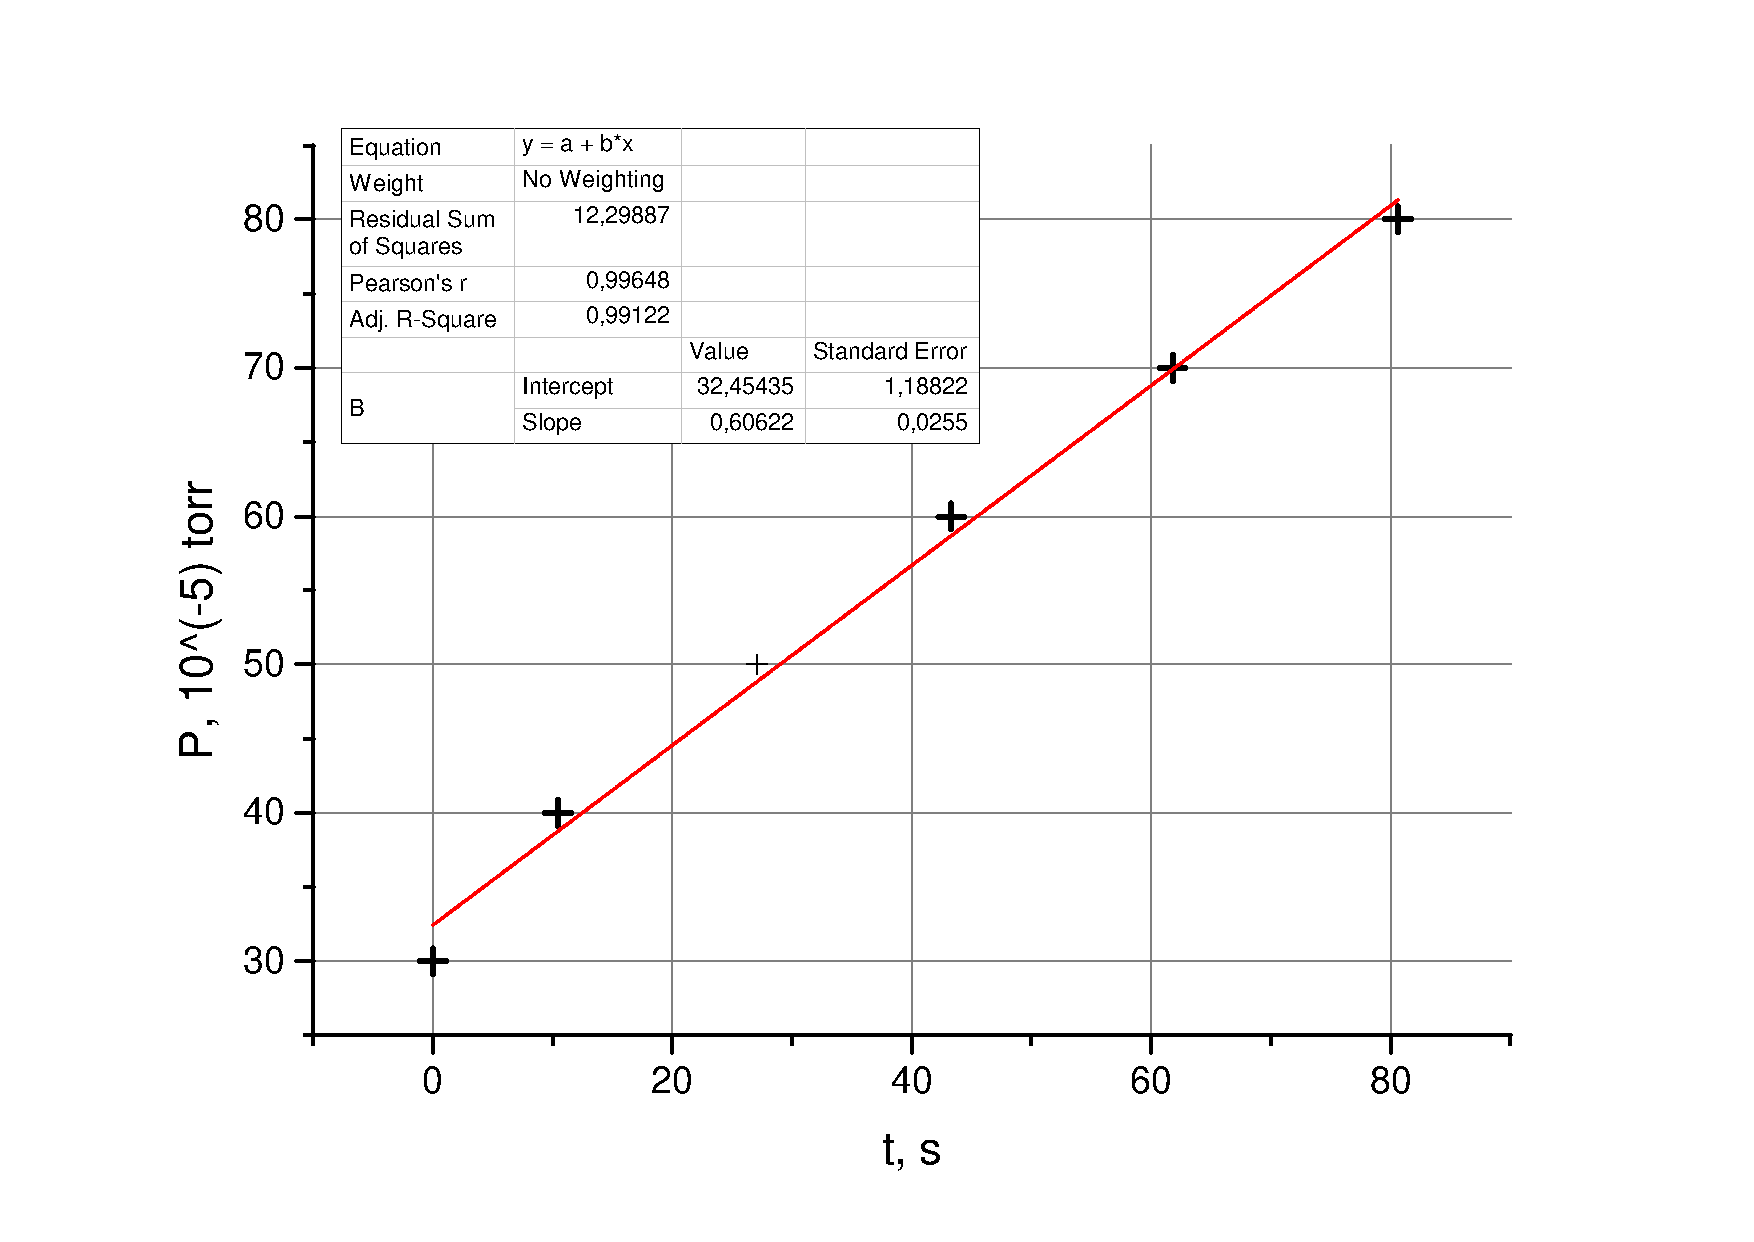
\includegraphics[width = 0.8\linewidth]{graph_1}
	
	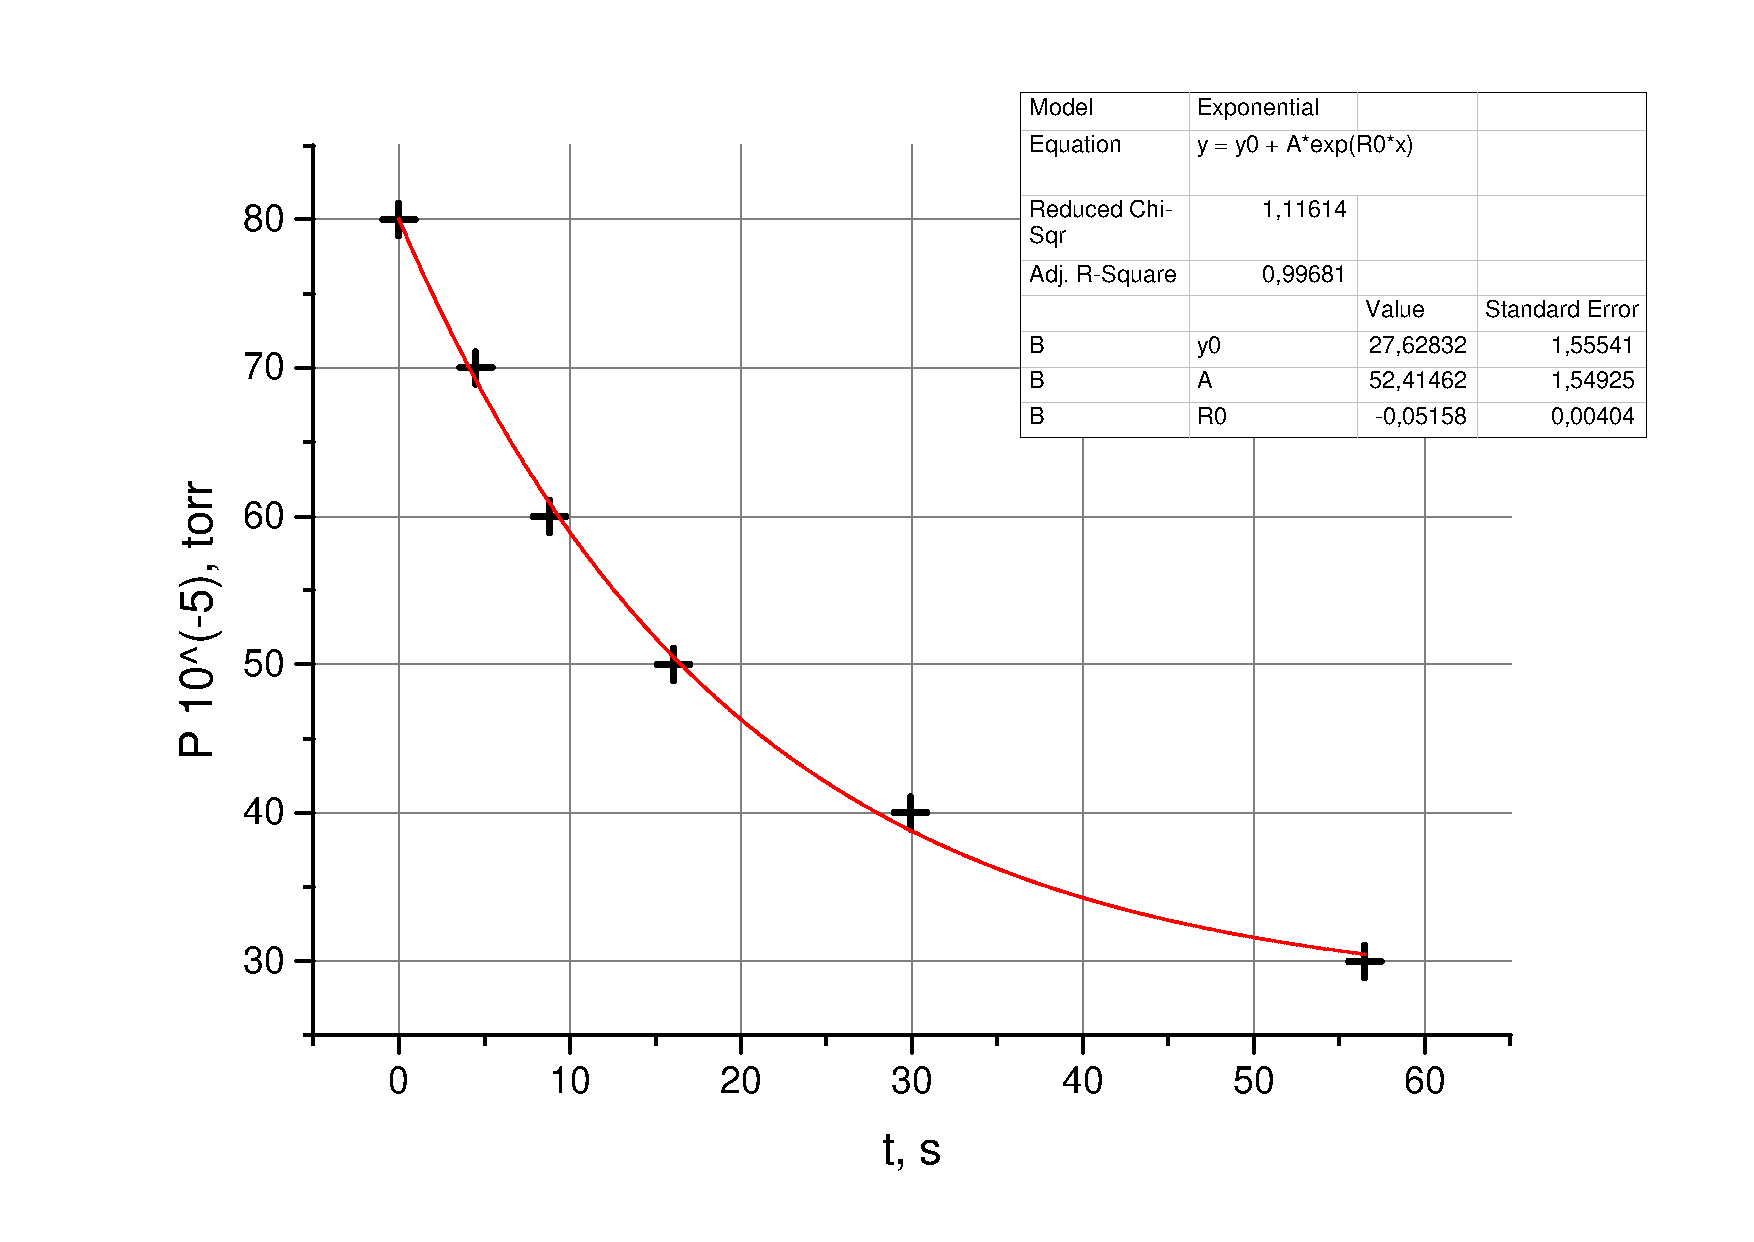
\includegraphics[width = 0.8\linewidth]{graph_2}
	
	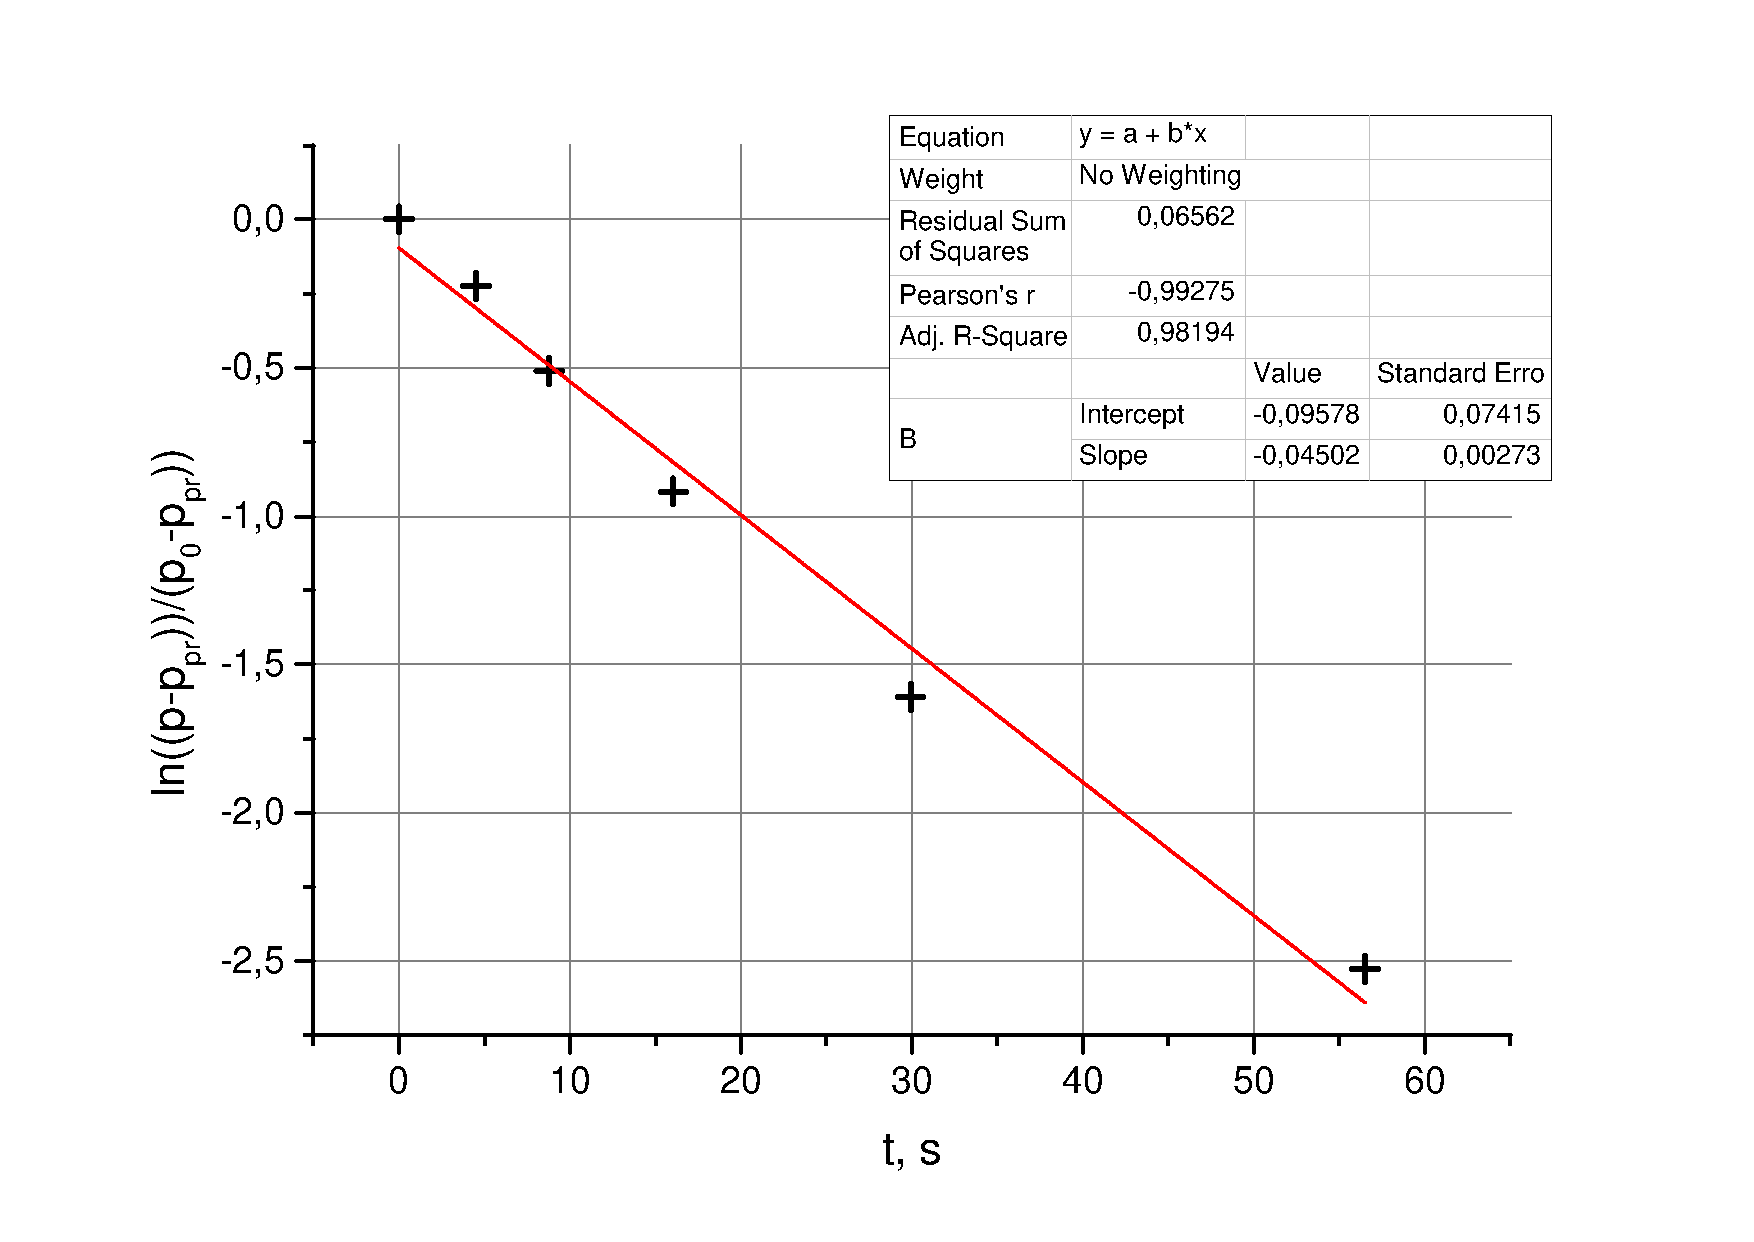
\includegraphics[width = 0.8\linewidth]{graph_3}
	
	Из графиков найдем скорость откачки: $ W = (13.4\pm 0.6)\cdot 10^{-2} \frac{\text{л}}{\text{с}}$.
	
	Оценим $Q_{\text{н}} \sim WP_{\text{пр}} - V_{\text{вв}}\frac{\dif P}{\dif t} =2.24 \cdot 10^{-5} \frac{\text{Торр}\cdot\text{л}}{\text{с}}$.
	
	
	\[
	P_{\text{пр}}W = Q_1, \quad P_{\text{уст}}W = Q_1 + \frac{\dif(PV)}{\dif t}
	\]
	
	\[
	W = \frac{\dif V}{\dif t} = \frac{\dif V}{\dif t} = \frac{4}{3}\frac{r^3}{L}\sqrt{\frac{2\pi RT}{\mu}} = 12.08 \pm 0.7 \, \frac{\text{л}}{\text{с}}
	\]
	Этот результат примерно совпадает с полученным в предыдущем пункте. 
	\section{Вывод}
		Получение вакуума, безусловно, интересный процесс. Мы научились получать и измерять высокий и низкий вакуум. Возможно, это понадобится.
\end{document}


